\documentclass[letterpaper, 10pt, conference]{ieeeconf}
\IEEEoverridecommandlockouts \overrideIEEEmargins
\usepackage{amsmath,amssymb,url,times,subfigure,graphicx,theorem}
\usepackage{graphicx,subfigure,hyperref}
\usepackage{color,comment}
\usepackage{csquotes}


\newcommand{\norm}[1]{\ensuremath{\left\| #1 \right\|}}
\newcommand{\abs}[1]{\ensuremath{\left| #1 \right|}}
\newcommand{\bracket}[1]{\ensuremath{\left[ #1 \right]}}
\newcommand{\braces}[1]{\ensuremath{\left\{ #1 \right\}}}
\newcommand{\parenth}[1]{\ensuremath{\left( #1 \right)}}
\newcommand{\ip}[1]{\ensuremath{\langle #1 \rangle}}
\newcommand{\refeqn}[1]{(\ref{eqn:#1})}
\newcommand{\reffig}[1]{Fig. \ref{fig:#1}}
\newcommand{\tr}[1]{\mbox{tr}\ensuremath{\negthickspace\bracket{#1}}}
\newcommand{\trs}[1]{\mbox{tr}\ensuremath{\!\bracket{#1}}}
\newcommand{\deriv}[2]{\ensuremath{\frac{\partial #1}{\partial #2}}}
\newcommand{\G}{\ensuremath{\mathsf{G}}}
\newcommand{\SO}{\ensuremath{\mathsf{S\mathcal O(3)}}}
\newcommand{\T}{\ensuremath{\mathsf{T}}}
\renewcommand{\L}{\ensuremath{\mathsf{L}}}
\newcommand{\so}{\ensuremath{\mathfrak{so}(3)}}
\newcommand{\SE}{\ensuremath{\mathsf{SE(3)}}}
\newcommand{\se}{\ensuremath{\mathfrak{se}(3)}}
\renewcommand{\Re}{\ensuremath{\mathbb{R}}}
\newcommand{\Sph}{\ensuremath{\mathsf{S}}}
\newcommand{\aSE}[2]{\ensuremath{\begin{bmatrix}#1&#2\\0&1\end{bmatrix}}}
\newcommand{\ase}[2]{\ensuremath{\begin{bmatrix}#1&#2\\0&0\end{bmatrix}}}
\newcommand{\D}{\ensuremath{\mathbf{D}}}
\renewcommand{\d}{\ensuremath{\mathbf{d}}}
\newcommand{\pair}[1]{\ensuremath{\left\langle #1 \right\rangle}}
\newcommand{\met}[1]{\ensuremath{\langle\!\langle #1 \rangle\!\rangle}}
\newcommand{\Ad}{\ensuremath{\mathrm{Ad}}}
\newcommand{\ad}{\ensuremath{\mathrm{ad}}}
\newcommand{\g}{\ensuremath{\mathfrak{g}}}
\newcommand{\argmin}{\operatornamewithlimits{argmin}}
\newcommand{\argmax}{\operatornamewithlimits{argmax}}

\title{\LARGE \bf
Autonomous Exploration by Expected Information Gain from Probabilistic Occupancy Grid Mapping
%Autonomous Exploration by Predictive Information Gain from Probabilisitic Occupancy Grid Mapping
%Autonomous Exploration by Predictive Occupancy Grid Mapping
%Autonomous Exploration by Predicting Occupancy Grid Maps
}

\author{Evan Kaufman, Taeyoung Lee, and Zhuming Ai%, and Ira S. Moskowitz%
\thanks{Evan Kaufman, Taeyoung Lee, Mechanical and Aerospace Engineering, George Washington University, Washington DC 20052 {\tt \{evankaufman,tylee\}@gwu.edu}}
\thanks{Zhuming Ai, Information Management \& Decision Architectures, U.S. Naval Research Laboratory,  Washington, DC 20375}
\thanks{This research has been supported by the U.S. Naval Research Laboratory Base Program ``Intelligent Microflyer'' and in part by NSF under the grants CMMI-1243000, CMMI-1335008, and CNS-1337722.}
}


\newcommand{\EditTL}[1]{{\color{red}\protect #1}}
\newcommand{\EditEK}[1]{{\color{blue}\protect #1}}

\newtheorem{definition}{Definition}
\newtheorem{lem}{Lemma}
\newtheorem{prop}{Proposition}
\newtheorem{cor}{Corollary}
\newtheorem{remark}{Remark}
\begin{document}



\maketitle
\thispagestyle{empty}
\pagestyle{empty}


%%%%%%%%%%%%%%%%%%%%%%%%%%%%%%%%%%%%%%%%%%%%%%%%%%%%%%%%%%%%%%%%%%%%%%%%%%%%%%%%
\begin{abstract}
Occupancy grid maps are spatial representations of environments, where the space of interest is decomposed into a number of cells that are considered either occupied or free. This paper focuses on exploring occupancy grid maps by predicting the uncertainty of the map. Based on recent improvements in computing occupancy probability, this paper presents a novel approach for selecting robot poses designed to maximize expected map information gain represented by the change in entropy. This result is simplified with several approximations to develop an algorithm suitable for real-time implementation. The predicted information gain proposed in this paper governs an effective autonomous exploration strategy when applied in conjunction with an existing motion planner to avoid obstacles, which is illustrated by numerical examples.
%The predicted information gain proposed in this paper, in conjunction with an existing motion planner to avoid obstacles, yield an effective autonomous exploration strategy, which is illustrated by numerical examples. 
\end{abstract}


%%%%%%%%%%%%%%%%%%%%%%%%%%%%%%%%%%%%%%%%%%%%%%%%%%%%%%%%%%%%%%%%%%%%%%%%%%%%%%%%
\section{Introduction}

Robotic mapping is the process of generating maps, which represent the environment in close proximity of a robot. The popular occupancy grid mapping representation provides information about the free and occupied space as the robot measures its surroundings~\cite{ThrBurFox05}. Occupancy grid mapping is commonly used while estimating robot location and orientation, known as simultaneous localization and mapping (SLAM). Several SLAM approaches are applied to a variety of problems when mobile robots traverse an environment to generate a map, but the robot actions assumed given (e.g.~\cite{ThrBurFox05,DurBai06,CheChe09}). A major problem is that generating an effective trajectory for the robot to follow would be unavailable knowing little or nothing about an environment. 
Autonomous exploration solves this problem, by choosing robotic motion through uncertain space, while building a map that is used for subsequent navigation~\cite{Yam97}.
In this paper, robotic motion is chosen to increase knowledge about the map; a robot chooses a trajectory designed to maximize the map information gain. % of the occupancy grid map.

A common approach to solve the autonomous exploration problem is known as frontier-based exploration, such as ~\cite{Yam97,Yam98}. This is the process of executing actions that move the robot toward the closest boundary between visited and unvisited space, known as a frontier.
Then the robot takes measurements at this location such that the mapped territory expands, and thus the new frontiers are pushed back. This process is repeated until the map is well-known.
Frontier-based exploration assumes that repeatedly moving toward the closest frontier and taking measurements are the best actions to gain new information about the map, though these systematic actions are not based on any consideration of the future uncertainty of the probabilistic map or optimality.
%there is no guarantee that these actions satisfy any optimality criteria.

%The uncertainty of an occupancy grid map is commonly measured with Shannon's entropy, which is a metric that measures map uncertainty.

Approaches aimed at determining the future uncertainty of an occupancy grid map commonly suffer from several approximations.
%Determining future occupancy grid map uncertainty requires predictive estimations, which suffer from several approximations. 
Most evident is that all approaches rely on inaccurate probabilistic occupancy grids. This mapping representation is typically based on heuristic approximations (e.g.~\cite{MorElf85,Elf89,ChoLynHutKanBurKavThr05,And09,PirRutBisSch11}) or simulated learning techniques \cite{ThrBurFox05,Thr01}. Map-based information gain is commonly determined with Shannon's entropy~\cite{StaGriBur05}, an uncertainty metric based on grid cell occupancy probability. Since this probability is heuristic or learned, any measure of entropy is subject to errors from approximated probability.
Furthermore, the expected entropy of an action is not directly calculated. Instead, these particle filter-based approaches assume expected entropy is equivalent to entropy based on expected measurement scans~\cite{JohStaPfaBur07}. This assumption is subject to inaccuracies due to the nonlinear nature of Shannon's entropy. %Furthermore, these approaches typically generate maps with a particle filter, which commonly require some tuning and may consume large amounts of onboard memory.

In this paper, we propose an autonomous exploration technique based on expected entropy change that avoids the aforementioned issues. 
%The occupancy grid mapping scheme is based on~\cite{KauLeeAiMos16}, which provides the exact solution of occupancy grid mapping of a single measurement ray. 
We develop a solution for expected entropy gain based on exact occupancy grid mapping~\cite{KauLeeAiMos16}. This solution directly calculates expected entropy from a probabilistic map based on similar assumptions of those applied to occupancy grid mapping.
Though more accurate than several other approaches, the proposed solution requires large computational resources, making real-time implementation difficult in certain scenarios.
Thus, we provide the tools to approximate the exact solution that reduces the computational requirements with realistic assumptions.
The motion of the robot is formulated as an optimization problem, where the expected entropy change is minimized, or equivalently the expected information gain is maximized.
Compared with the recent results (e.g. [12], [13], [16], [17]) that employ Rao-Blackwellized particle filters to deal with localization and autonomous exploration simultaneously with an approximate entropy change, this paper is based on an accurate solution to map information gain, under the assumption that the robot pose is known. In short, this paper presents an accurate and computationally-efficient approach to predict
map information gain for autonomous exploration with a novel structure that avoids common assumptions of the inverse sensor model and approximations of entropy change.



The paper is organized as follows. The problem is formulated in Section II. The exact solution to the expected uncertainty due to an individual 1D measurement is derived in Section III, along with optional approximations. The concept of entropy is extended to 2D autonomous exploration with a numerical example in Section IV, followed by conclusions.

%\begin{itemize}
%%	\item Introductory Paragraph
%%	\begin{itemize}
%%		\item Motivation for mapping
%%		\item Background on occupancy grid mapping
%%		\item Background on SLAM and shortfall of SLAM: trajectory is assumed known
%%	\end{itemize}
%	\item Related research
%	\begin{itemize}
%		\item Motion planning: moving toward a goal assuming a map is known
%		\item If map is unknown: frontier-based autonomous exploration
%		\item Problematic assumption: moving toward uncertain space will yield high information gain
%	\end{itemize}
%	\item Proposed approach
%	\begin{itemize}
%		\item Description of Shannon Entropy
%		\item Focus on how we expect the entropy to \emph{change} rather than just its current value
%		\item Work builds largely off contributions in exact inverse sensor models
%		\item Goal: design a computationally-efficient approach to choose a robot pose based on predicting map information gain
%	\end{itemize}
%\end{itemize}



%%%%%%%%%%%%%%%%%%%%%%%%%%%%%%%%%%%%%%%%%%%%%%%%%%%%%%%%%%%%%%%%%%%%%%%%%%%%%%%%
\section{Problem Formulation}

\subsection{Occupancy Grid Mapping}

Let a map $m$ be decomposed into $n_m$ evenly-spaced 2D grid cells, where the $i$-th grid cell is assigned to a static binary random variable $\mathbf{m}_i$ for $i\in\braces{1,2,...,n_m}$, that is defined as $\mathbf{m}_i=1$ when occupied, and $\mathbf{m}_i=0$ when free. The location and size of each grid cell is assumed known. Therefore, a map $m$ is defined by $\{\mathbf{m}_1,\mathbf{m}_2,\ldots, \mathbf{m}_{n_m}\}$, and there are $2^{n_{m}}$ possible maps. 

Another random variable is defined as $\bar{\mathbf{m}}_i=1-\mathbf{m}_i$ for convenience. The probability that the $i$-th cell is occupied is $P(\mathbf{m}_i)$, and the probability that it is free is $P(\bar{\mathbf{m}}_i)=1-P(\mathbf{m}_i)$. The random variables $\mathbf{m}_i$ are assumed as mutually independent variables, i.e.,
\begin{align}
P(m)=P(\mathbf{m}_1,\mathbf{m}_2,...,\mathbf{m}_{n_m})=\prod_{i=1}^{n_m}P(\mathbf{m}_i).
\end{align}

%Occupancy grid mapping produces a probabilistic map; none of the $n_m$ grid cell occupancies are completely certain.
Occupancy grid mapping is the process of determining these probabilities based on robot poses and measurement scans. 
More explicitly, let $t$ be a discrete variable for time. The $t$-th pose is denoted $X_t=\braces{x_t,R_t}$, where the planar position and direction of the robot at $t$ are denoted by $x_t\in\Re^2$ and $R_t\in\Sph^1=\braces{q\in\Re^2|\norm{q}=1}$, i.e., the attitude corresponds to a direction on a 2D plane. 
%the robot position $x_t\in\Re^2$ and attitude $R_t\in\Sph^1$ are confined to a 2D plane such that $\Sph^1=\braces{q\in\Re^2|\norm{q}=1}$.
 Let $X_{1:t}$ denote the history of poses from the initial time to the current time, i.e., $X_{1:t}=\{X_1,X_2,\ldots, X_t\}$. At each pose, the robot receives a 2D measurement \emph{scan}, composed of $n_z$ measurement \emph{rays}. These rays are 1D depth measurements of known direction from the current pose to the closest occupied space, subject to a known \emph{forward sensor model} $p(z_{t,l}|m,X_t)$, where $z_{t,l}$ is the $l$-th measurement ray of the $t$-th scan $Z_t=\braces{z_{t,1},z_{t,2},\ldots,z_{t,n_z}}$ and $Z_{1:t}$ is the measurement history. 
%More explicitly, let the $t$-th measurement \emph{scan} be composed of $n_z$ measurement \emph{rays}, i.e., $Z_t=\braces{z_{t,1},z_{t,2},\ldots,z_{t,n_z}}$, so the measurement scan history is $Z_{1:t}=\{Z_1,Z_2,\ldots, Z_t\}$. 

The goal of occupancy grid mapping is to obtain the \emph{inverse sensor model} $P(\mathbf{m}_i|X_{1:t},Z_{1:t})$ for all grid cells inside the sensor field of view.
Suppose that the inverse sensor model before $t$-th time step is given, namely $P(m|X_{1:t-1},Z_{1:t-1})$, and the $l$-th measurement ray $z_{t,l}$ is available from pose $X_t$.
The inverse sensor model due to $z_{t,l}$ at the $t$-th time step follows Bayes' rule,
\begin{align}
\label{eqn:BayesRuleRayISM}
P(&m|z_{t,l},X_{1:t},Z_{1:t-1})\nonumber
\\
&=\frac{p(z_{t,l}|m,X_{1:t},Z_{1:t-1})P(m|X_{1:t-1},Z_{1:t-1})}{p(z_{t,l}|X_{1:t},Z_{1:t-1})}\nonumber
\\
&=\eta_{t,l}p(z_{t,l}|m,X_{1:t},Z_{1:t-1})P(m|X_{1:t-1},Z_{1:t-1}),
\end{align}
where $\eta_{t,l}$ is a normalizing constant independent of $m$, and we used the fact that $X_t$ carries no information about $m$ without $z_{t,l}$. However, $P(\mathbf{m}_i|z_{t,l},X_{1:t},Z_{1:t-1})$ is perceived as intractable because the exact solution considers every combination of map $m$ to obtain the normalizer $\eta_{t,l}$, yielding $\mathcal O(2^{n_m})$ per grid cell. This is why heuristic solutions based on learning or intuition substitute the inverse sensor model. Recently, \refeqn{BayesRuleRayISM} was solved computationally-efficiently to obtain an exact solution in real-time~\cite{KauLeeAiMos16}, summarized next.

Consider a reduced map, namely $r_l$, composed of only $n_{r,l}$ grid cells that the $l$-th measurement ray intersects, indexed by increasing distance from the robot. Let the $k$-th cell of $r_l$, namely $\mathbf{r}_{l,k}$, correspond to $\mathbf{m}_i$, i.e., $\mathbf{r}_k=\mathbf{m}_i$ and $\bar{\mathbf{r}}_k=\bar{\mathbf{m}}_i$.
From~\cite{KauLeeAiMos16}, the inverse sensor model of the individual grid cell $\mathbf{m}_i$ is
\begin{align}
\label{eqn:InvSenModWithProbDens}
&P(\mathbf{m}_i|z_{t,l},X_{1:t},Z_{1:t-1})\nonumber
\\
&=\eta_{t,l}
P(\mathbf{r}_{l,k}|X_{1:t-1},Z_{1:t-1})\nonumber\\
&\quad\times \bigg[\sum_{i=1}^{k-1}\bigg\{\prod_{j=0}^{i-1}P(\bar{\mathbf{r}}_{l,j}|X_{1:t-1},Z_{1:t-1})\bigg\}\nonumber\\
&\quad\times p(z_{t,l}|\mathbf{r}_{l,i+},X_t)P(\mathbf{r}_{l,i}|X_{1:t-1},Z_{1:t-1})\nonumber\\
&\quad + \bigg\{\prod_{j=0}^{k-1}P(\bar{\mathbf{r}}_{l,j}|X_{1:t-1},Z_{1:t-1})\bigg\}p(z_{t,l}|\mathbf{r}_{l,k+},X_t)
\bigg],
\end{align}
where $\mathbf{r}_{l,k+}$ corresponds to all $r_l$ such that cells with index less than $k$ are free, the $k$-th cell is occupied, and cells with greater index are irrelevant. Put differently, the $k$-th cell is the closest occupied cell along the $l$-th ray. The normalizer used in \refeqn{InvSenModWithProbDens} is defined as
\begin{align}
\label{eqn:allEta}
\eta_{t,l}
&=
\bigg[\sum_{i=1}^{n_{r,l}+1}\bigg\{\prod_{j=0}^{i-1}P(\bar{\mathbf{r}}_{l,j}|X_{1:t-1},Z_{1:t-1})\bigg\}\nonumber\\&\quad\times p(z_{t,l}|\mathbf{r}_{l,i+},X_t)P(\mathbf{r}_{l,i}|X_{1:t-1},Z_{1:t-1})\bigg]^{-1}.
\end{align}
This approach to obtain the inverse sensor model is advantageous because of computational efficiency and accuracy, obtaining the exact solution in $\mathcal O(n_{r,l}+1)$ operations for \emph{all} grid cells visible by this measurement ray. In occupancy grid mapping, one may use \refeqn{InvSenModWithProbDens} and \refeqn{allEta} in real-time to avoid common approximations or learned solutions.

\subsection{Shannon's Entropy and Map Information}

Since occupancy grid mapping provides a probabilistic representation of surrounding space, this mapping scheme holds probabilistic information about the uncertainty of the map. Shannon's entropy is commonly used as a measure of uncertainty, such as in~\cite{StaGriBur05}. Given the probabilities of each grid cell of map $m$, Shannon's entropy is defined as the sum of the entropy of each cell,
\begin{align}
\label{eqn:ShannonsEntropyDef}
H(&P(m))=\nonumber\\&-\sum_{i=1}^{n_m}\braces{
P(\mathbf{m}_i)\log{P(\mathbf{m}_i})+P(\bar{\mathbf{m}}_i)\log{(P(\bar{\mathbf{m}}_i}))}.
\end{align}
The entropy of the $i$-th grid cell is maximized when $P(\mathbf{m}_i)=0.5$ (greatest uncertainty) and minimized when $P(\mathbf{m}_i)\in\braces{0,1}$ (smallest uncertainty). %; thus Shannon's entropy is a measure of uncertainty.

%\begin{itemize}
%	\item Define the entropy, and describe uncertainty metric meaning
%	\item Entropy can be calculated much more accurately than prior work now that a computationally-efficient exact inverse sensor model is available
%\end{itemize}

\subsection{Autonomous Exploration}

The goal of autonomous exploration is to determine future poses that maximize the map information gain, or equivalently minimize the map entropy. 
%Let the objective function from the first time step $t=1$ to the $t_f$-th time step be
%\begin{align}
%\label{eqn:ObjFun}
%\mathcal I(X_{2:t_f})&=H(P(m|X_{1},Z_{1}))\nonumber\\&\quad-\text{E}\left[H(P(m|X_{1:t_f},Z_{1:t_f}))\right].
%\end{align}
Since autonomous exploration is conducted in uncertain environments, a complete trajectory cannot be known before a priori.
Instead, an objective function governs the motion between intermediate poses, building an occupancy grid map along the way.

Suppose at time $t$, $P(m|X_{1:t},Z_{1:t})$ is given. Let $X_c$ be the pose of the robot after the $t$-th time step.
The expected information gain $\mathcal I(X_c)$ is defined as the negative change
\begin{align}
\label{eqn:ObjFun}
\mathcal I(X_c)&=H(P(m|X_{1:t},Z_{1:t}))\nonumber\\&\quad-\text{E}\left[H(P(m|X_{1:t},Z_{1:t},X_c,Z_c))\right],
\end{align}
where $H(P(m|X_{1:t},Z_{1:t}))$ may be computed with \refeqn{ShannonsEntropyDef} and $\text{E}\left[H(P(m|X_{1:t},Z_{1:t},X_c,Z_c))\right]$ is the expected entropy with robot pose $X_c$ and the expectation is taken over $Z_c$.
Since autonomous exploration is formulated as a trajectory optimization, the goal is to repeatedly choose optimal $X_c^*$ that maximizes the objective function
\begin{align}
\label{eqn:Objective}
X_c^*=\argmax_{X_c}{\mathcal I(X_c)},
\end{align}
avoiding collisions by satisfying the inequality constraint
\begin{align}
\label{eqn:CollisionInequalityConstraint}
P_\text{collision}(X)=1-\prod_{i\in\mathcal C_X}(P(\bar{\mathbf{m}}_i|X_{1:t},Z_{1:t})\leq\beta,
\end{align}
where $\mathcal C_X$ is the set of grid cells falling inside a volume of preselected size around $X$ that may cause collision and $\beta>0$ is a small acceptable probability of collision.
Once the robot has translated to $X_c^*$, the above process is repeated.
%Once the trajectory satisfying \refeqn{CollisionInequalityConstraint} between $X_t$ and $X_c$ is completed, the greedy process is repeated with an updated map.


\section{1D Ray Expected Information Gain}

The expected entropy from an individual measurement ray from a known pose is presented, based on the exact solution to occupancy grid mapping from~\cite{KauLeeAiMos16}.

\subsection{Single Ray Expected Value of Entropy}
We consider the expected entropy due to the $l$-th measurement ray $z_{c,l}$ at position $x_c$,
\begin{align}
\label{eqn:HRayInt}
\text{E}[H(P(m|&X_{1:t},Z_{1:t},x_c,z_{c,l}))]
\nonumber\\&
=\int_{z_\text{min}}^{z_\text{max}}
H(P(m|X_{1:t},Z_{1:t},x_c,z_{c,l}))\nonumber\\&\qquad\quad\times p(z_{c,l}|X_{1:t},Z_{1:t},x_c)
dz_{c,l}.
\end{align}
%where $z_\text{min}$ and $z_\text{max}$ are sensor limits. Considering the continuous space of possible measurements of $z_{c,l}$ would make \refeqn{HRayInt} intractable to calculate. Thus, w
We discretize the measurement ray space such that $z_{c,l}$ falls on points along the measurement ray intersecting with grid cell edges.
The discretized expected value of \refeqn{HRayInt} is
\begin{align}
\label{eqn:DiscExpEntropyRay}
\text{E}[H(P(m|&X_{1:t},Z_{1:t},x_c,z_{c,l}))]
\nonumber\\&=\sum_{k=1}^{n_{r,l}+1}\bigg\{H(P(m|X_{1:t},Z_{1:t},x_c,z_{c,l,k}))\nonumber\\&\qquad\qquad\times P(z_{c,l,k}|X_{1:t},Z_{1:t},x_c)\bigg\},
\end{align}
where index $z_{c,l,k}$ is the distance from $x_c$ to the $k$-th grid cell of the $l$-th reduced map $r_l$, known from geometry.

Standing alone, the term $P(z_{c,l,k}|X_{1:t},Z_{1:t},x_c)$ from \refeqn{DiscExpEntropyRay} has a convoluted meaning because the depth $z_{c,l,k}$ does not directly depend on the map. However, we present a method to obtain this discretized probability. %Despite how this term is replaced with a normalizer in ~\cite{ThrBurFox05} replaces
Following the assumption that $z_{c,l}$ is discretized to known distances, the probabilities are proportional to their densities, as the area under the density curve is infinitesimal and fixed. Accounting for all cases, the probability is
\begin{align}
\label{eqn:ProbWithDelta}
P(z_{c,l,k}|X_{1:t},Z_{1:t},x_c)=\frac{p(z_{c,l,k}|X_{1:t},Z_{1:t},x_c)}{\sum_{i=1}^{n_{r,l}+1}p(z_{c,l,i}|X_{1:t},Z_{1:t},x_c)}.
\end{align}
Conveniently, this density corresponds to the inverse normalizer defined in \refeqn{BayesRuleRayISM} as the denominator from Bayes' rule,
\begin{align}
\label{eqn:DiscretizedProb}
p(z_{c,l,k}|X_{1:t},X_c,Z_{1:t})=\eta_{c,l,k}^{-1},
\end{align}
where $\eta_{c,l,k}^{-1}$ is defined in \refeqn{allEta}. However, instead of evaluating the $t$-th pose $X_t$ and measured ray $z_{t,l}$, we simply consider $X_c$ and ray depth $z_{c,l,k}$ based on histories $X_{1:t}$ and $Z_{1:t}$ to obtain the inverse normalizer,
\begin{align}
\label{eqn:allEtaAtC}
\eta_{c,l,k}^{-1}
&=
\sum_{i=1}^{n_{r,l}+1}\bigg\{\prod_{j=0}^{i-1}P(\bar{\mathbf{r}}_{l,j}|X_{1:t},Z_{1:t})\bigg\}\nonumber\\&\qquad\times p(z_{c,l,k}|\mathbf{r}_{l,i+},X_c)P(\mathbf{r}_{l,i}|X_{1:t},Z_{1:t}).
\end{align}
By substituting \refeqn{ProbWithDelta} and \refeqn{DiscretizedProb} into \refeqn{DiscExpEntropyRay}, the expected entropy at $X_c$ from individual measurement ray $z_{c,l}$ is
\begin{align}
\label{eqn:HRayComplete}
&\text{E}[H(P(m|X_{1:t},Z_{1:t},x_c,z_{c,l}))]=\left(\sum_{i=1}^{n_{r,l}+1}\eta_{c,l,i}^{-1}\right)^{-1}\nonumber\\&\quad\quad\times\sum_{k=1}^{n_{r,l}+1}\bigg\{H(P(m|X_{1:t},Z_{1:t},x_c,z_{c,l,k}))\eta_{c,l,k}^{-1}\bigg\},
\end{align}
where $\eta_{c,l,k}^{-1}$ is taken from \refeqn{allEtaAtC}.
Here, \refeqn{HRayComplete} provides the expected entropies for cells inside the field of view of $r_l$. %; cells outside this reduced map are trivially changed by $0$ due to $z_{c,l}$.
The entropies of cells outside the field of view remain unchanged.

%, and $z_{c,l,n_{r,l}+1}=z_\text{max}$ such that
%\begin{align}
%\label{eqn:SumDiscretizedMeasRay}
%\sum_{k=1}^{n_{r,l}+1}P(z_{c,l,k}|X_{1:t},Z_{1:t},x_c)=1,
%\end{align}
%to account for every case on the reduced map.
%
%It is commonly thought that the probability of a future measurement, in this case $P(z_{c,l,k}|X_{1:t},Z_{1:t},x_c)$, is too difficult to calculate. As part of the inverse sensor model, the probability density $p(z_{c,l,k}|X_{1:t},Z_{1:t},x_c)$ is absorbed in the normalizer, and typically neglected from further investigation~\cite{ThrBurFox05}. However, the $k$-th normalizer, namely $\eta_{c,l,k}$, is easily obtained with \refeqn{allEta}, and this holds important information.
%From \refeqn{BayesRuleRayISM}, evaluating $z_{c,l}$ now after the $t$-th time step we have
%\begin{align}
%\label{eqn:DiscretizedProb}
%p(z_{c,l,k}|X_{1:t},X_c,Z_{1:t})={\eta_{c,l,k}}^{-1}.
%\end{align}
%%\begin{align}
%%\label{eqn:DiscretizedProb}
%%P(z_{c,l,k}|X_{1:t},X_c,Z_{1:t})=\frac{\delta z}{\eta_{c,l,k}},
%%\end{align}
%%from \refeqn{BayesRuleRayISM} where $\delta z$ represents an infinitisimal width such that $\delta z\ll\alpha$. 
%Following the assumption that $z_{c,l}$ is restricted to cell edges and a maximum reading, the probabilities are proportional to their densities, as the area under the density curve is infinitesimal and fixed. Accounting for all cases, the probability is
%\begin{align}
%\label{eqn:ProbWithDelta}
%P(z_{c,l,k}|X_{1:t},Z_{1:t},x_c)=\frac{p(z_{c,l,k}|X_{1:t},Z_{1:t},x_c)}{\sum_{i=1}^{n_{r,l}+1}p(z_{c,l,i}|X_{1:t},Z_{1:t},x_c)},
%\end{align}
%which may be written in terms of normalizers as
%\begin{align}
%\label{eqn:PRayFromEta}
%P(z_{c,l,k}|X_{1:t},Z_{1:t},x_c)=\frac{\eta_{c,l,k}^{-1}}{\sum_{i=1}^{n_{r,l}+1}{\eta_{c,l,i}}^{-1}}.
%\end{align}

%The expected entropy from candidate pose $X_c$ with measurement ray $z_{c,l}$ is obtained with \refeqn{DiscExpEntropyRay} and \refeqn{PRayFromEta}, where the normlizers come from \refeqn{allEta}. The ray inverse sensor model \refeqn{InvSenModWithProbDens} provides the probabilities of the reduced map $r_l$, and all cells outside of $r_l$ remain unchanged. Thus, grid cells outside $r_l$ need not be considered in either term of the objective function \refeqn{ObjFun} with respect to $x_c$ and $z_{c,l}$.
%
%Let $k_\text{c}$ be an index corresponding to a cell along a measurement ray and let $k_\text{m}$ be an index corresponding to a measurement along a measurement ray. 
%Let the objective function of the $l$-th measurement ray \emph{only} be denoted $\mathcal I_\text{ray}(x_c,z_{c,l})$.
%Then, the objective function from \refeqn{ObjFun} is simplified to include just the grid cells intersecting along the ray as
%\begin{align}
%\label{eqn:ObjFunRayComplete}
%&\mathcal I_\text{ray}(x_c,z_{c,l})\nonumber\\&=\sum_{k_\text{c}=1}^{n_{r,l}+1}\bigg[H(P(\mathbf{r}_{c,l,k_\text{c}}|X_{1:t},Z_{1:t}))\nonumber\\
%&\quad
%-\sum_{k_\text{m}=1}^{n_{r,l}+1}\bigg( H(P(\mathbf{r}_{c,l,k_\text{c}}|X_{1:t},Z_{1:t},x_c,z_{c,l,k_\text{m}}))\nonumber\\
%&\quad\quad\quad\quad\quad\quad\quad\times P(z_{c,l,k_\text{m}}|X_{1:t},Z_{1:t},x_{c})\bigg)
%\bigg].
%\end{align}

%\subsection{Full Scan Expected Value of Entropy}

\subsection{Approximation of Expected Ray Entropy}

The order of computation for each measurement ray is $\mathcal O((n_{r,l}+1)^2)$ since the summations of \refeqn{allEtaAtC} are embedded in \refeqn{HRayComplete}. However, several of those intersections provide negligible information since the probability of the $l$-th measurement ray capturing certain cell depths is close to zero.

The approximation of expected ray entropy provides a method to reduce the computation of \refeqn{allEtaAtC} substantially by systematically selecting a smaller set of grid cells to consider over the summations of \refeqn{allEtaAtC} and \refeqn{HRayComplete}.
The smaller set is determined by the detection probability, or the probability that a particular cell is captured by the measurement ray, %These cells correspond to the $\hat n$ cells with the greatest probabilities of being captured by the measurement ray, known as the detection probability. This can be found recursively as
%
%select the terms that contribute
%We systematically select a limited number of terms that affect
%
%
%The large order of computation is reduced substantially by lowering the summation limits of \refeqn{allEtaAtC} and \refeqn{HRayComplete}. Consider the $\hat{n}$ intersections of $r_l$ with the greatest probability of returning a measurement. The detection probability is found recursively as
\begin{align}
\label{eqn:ProbOfFirstCell}
&P(\mathbf{r}_{l,k+}|X_{1:t},Z_{1:t})\nonumber\\&=\bigg\{\prod_{j=0}^{k-1}P(\bar{\mathbf{r}}_{l,j}|X_{1:t},Z_{1:t})\bigg\}P(\mathbf{r}_{l,k}|X_{1:t},Z_{1:t}),
\end{align}
which is the probability that $\mathbf{r}_{l,k}$ is the closest occupied grid cell based on past poses and measurement scans, independent of cells beyond the $k$-th cell from $x_c$.
Let $\hat n>0$ be a fixed number of grid cells for all rays such that $\hat n\leq n_{r,l}+1$ for all $l$.
Let $\hat{r}_{l}$ correspond to grid cells that yield the $\hat{n}$ maximum values \refeqn{ProbOfFirstCell} (the $\hat n$ most likely ray detections), indexed by increasing distance from candidate location $x_c$.
By replacing the reduced map $r_l$ with $\hat{r}_l$ and changing the summation limits to $\braces{1,2,...,\hat n}$ in \refeqn{allEtaAtC} and \refeqn{HRayComplete}, the order of computation is reduced to $\mathcal O({\hat{n}}^2)$.
Even though $n_{r,l}$ is different among various rays in general, $\hat n$ is fixed, which fixes the computational order.
In short, this method reduces the required computation substantially by systematically neglecting those grid cells with little effect.
%When $\hat n=n_{r,l}+1$, the ray objective function is computed without approximation.
%
%
%Then, the objective function \refeqn{ObjFunRayComplete} from this measurement ray is approximated as
%\begin{align}
%\label{eqn:ObjFunRayApprox}
%&\mathcal I_\text{ray}_\text{approx}(x_c,z_{c,l})\nonumber\\&=\sum_{k_\text{c}=1}^{\hat{n}}\bigg[H(P(\hat{\mathbf{r}}_{c,l,k_\text{c}}|X_{1:t},Z_{1:t}))\nonumber\\
%&\quad
%-\sum_{k_\text{m}=1}^{\hat{n}}\bigg( H(P(\hat{\mathbf{r}}_{c,l,k_\text{c}}|X_{1:t},Z_{1:t},x_c,\hat{z}_{c,l,k_\text{m}}))\nonumber\\
%&\quad\quad\quad\quad\quad\quad\quad\times P(\hat{z}_{c,l,k_\text{m}}|X_{1:t},Z_{1:t},x_{c})\bigg)
%\bigg],
%\end{align}
%where $\hat{z}_{c,l,k_\text{m}}$ is the expected measurement distance from $x_c$ to $\hat{\mathbf{r}}_{k_\text{m}}$, known from geometry. This measurement probability comes from \refeqn{PRayFromEta} over a smaller set,
%\begin{align}
%\label{eqn:ApproxSimplifiedPRayFromEta}
%P(\hat{z}_{c,l,k_\text{m}}|X_{1:t},x_{c},Z_{1:t})=\frac{\hat{\eta}_{c,l,k_\text{m}}^{-1}}{
%\sum_{i=1}^{\hat{n}}
%\hat{\eta}_{c,l,i}^{-1}
%},
%\end{align}
%where the normalizer is extended from \refeqn{allEta} as
%\begin{align}
%\label{eqn:SimplifiedAllEta}
%\hat{\eta}_{c,l,k_\text{m}}
%&=
%\bigg[\sum_{i=1}^{\hat{n}}\bigg\{\prod_{j=0}^{i-1}P(\hat{\bar{\mathbf{r}}}_{c,l,j}|X_{1:t},Z_{1:t})\bigg\}\nonumber\\&\times p(\hat{z}_{c,l,k_\text{m}}|\hat{\mathbf{r}}_{c,l,i+},x_c)P(\hat{\mathbf{r}}_{l,i}|X_{1:t},Z_{1:t})\bigg]^{-1}, 
%\end{align}
%and the inverse sensor model from \refeqn{InvSenModWithProbDens} is
%\begin{align}
%\label{eqn:SimplifiedInvSenModWithProbDens}
%&P(\hat{\mathbf{r}}_{c,l,k_\text{c}}|X_{1:t},Z_{1:t},x_c,\hat{z}_{c,l,k_\text{m}})\nonumber
%\\
%&=\hat{\eta}_{c,l,k_\text{m}}
%P(\mathbf{r}_{c,l,k_\text{c}}|X_{1:t},Z_{1:t})\nonumber\\
%&\quad\times \bigg[\sum_{i=1}^{k_\text{c}-1}\bigg\{\prod_{j=0}^{i-1}P(\hat{\bar{\mathbf{r}}}_{c,l,j}|X_{1:t},Z_{1:t})\bigg\}\nonumber\\
%&\quad\times p(z_{c,l,k_\text{m}}|\hat{\mathbf{r}}_{c,l,i+},X_t)P(\hat{\mathbf{r}}_{c,l,i}|X_{1:t},Z_{1:t})\nonumber\\
%&\quad + \bigg\{\prod_{j=0}^{k_\text{c}-1}P(\hat{\bar{\mathbf{r}}}_{c,l,j}|X_{1:t},Z_{1:t})p(z_{c,l,k_\text{m}}|\mathbf{r}_{l,k+},x_c)\bigg\}
%\bigg].
%\end{align}
%In short, the $\hat{n}$ grid cells with greatest detection probabilities from \refeqn{ProbOfFirstCell} serve as the only indices to obtain the approximate objective function $\mathcal I_\text{ray}_\text{approx}(x_c,z_{c,l})$ from \refeqn{ObjFunRayApprox}, which uses \refeqn{ApproxSimplifiedPRayFromEta}--\refeqn{SimplifiedInvSenModWithProbDens}. While a small amount of information is lost by neglecting grid cells that are unlikely to be detected, the required computation is reduced to $\mathcal O(\hat{n}^2)$ where $\hat{n}\ll n_{r,l}+1$. This approximation is justified with Monte Carlo numerical results.
%

\subsection{1D Ray Expected Information Gain Algorithm}

We present an algorithm pseudocode providing the necessary steps to obtain the objective function for a single measurement ray (Table \ref{tab:RayExpectedEntropyGain}). The variable $a_\text{temp}$ is an intermediate variable designed to avoid repeated calculations.
Fixed indices and condition variables are removed for simplification.

\begin{table}
\begin{tabular}{ l }
  Function: $\mathcal I_\text{ray}=\text{RayExpInfoGain}(x,P(r),z_{1:n_{r,l}})$\\
  Define $P(\bar{\mathbf{r}}_{0})=P(\bar{\mathbf{r}}_{n_{r,l}+1})=1$;\\
  for $k = 1,2,\ldots,n_{r,l}+1$\\
   \ \ $P(\mathbf{r}_{k+}) = P(\bar{\mathbf{r}}_{0:k-1})P(\mathbf{r}_{k})$;\\
   \ \ $P(\bar{\mathbf{r}}_{0:k})=P(\bar{\mathbf{r}}_{0:k-1})P(\bar{\mathbf{r}}_{k})$;\\
  end for\\
%  $P(\mathbf{r}_{(n_{r}+1)+}) = P(\bar{\mathbf{r}}_{0:n_{r}})$;\\
  Find $\hat r\subset r$ corresponding to the $\hat n$ greatest values of\\
  $\braces{P(\mathbf{r}_{1+}),P(\mathbf{r}_{2+}),\ldots,P(\mathbf{r}_{(n_{r,l}+1)+})}$;\\
  Define $P(\hat{\bar{\mathbf{r}}}_{0})=1$;\\
  for $k = 1,2,\ldots,\hat{n}$\\
   \ \ $P(\hat{\mathbf{r}}_{k+}) = P(\hat{\bar{\mathbf{r}}}_{0:k-1})P(\hat{\mathbf{r}}_{k})$;\\
   \ \ $P(\hat{\bar{\mathbf{r}}}_{0:k})=P(\hat{\bar{\mathbf{r}}}_{0:k-1})P(\hat{\bar{\mathbf{r}}}_{k})$;\\
  end for\\
  for $k_\text{m}=1,2,\ldots,\hat n$\\
   \ \ Initialize $\eta^{-1}_{k_\text{m}}=0$;\\
   \ \ for $k_\text{c}=1,2,\ldots,\hat n$\\
   \ \ \ \ $a_\text{temp}=P(\hat{\mathbf{r}}_{k_\text{c}+})p(z_{k_\text{m}}|\hat{\mathbf{r}}_{k_\text{c}+},x)$;\\
   \ \ \ \ $\tilde P(\hat{\mathbf{r}}_{k_\text{c}}|x,z_{k_\text{m}})=P(\hat{\mathbf{r}}_{k_\text{c}})\eta^{-1}_{k_\text{m}}+a_\text{temp}$;\\
   \ \ \ \ $\eta^{-1}_{k_\text{m}}=\eta^{-1}_{k_\text{m}}+a_\text{temp}$;\\
   \ \ end for\\
   \ \ $P(\hat{\mathbf{r}}_{k_\text{c}}|x,z_{k_\text{m}})=\eta_{k_\text{m}}\tilde P(\hat{\mathbf{r}}_{k_\text{c}}|x,z_{k_\text{m}})$ for all $k_\text{c}=1,2,\ldots,\hat n$;\\
   end for\\ 
   $P(z_{k_\text{m}}|x)=\frac{\eta^{-1}_{k_\text{m}}}{\sum_{i=1}^{\hat n}\eta^{-1}_{i}}$ for $k_\text{m}=1,2,\ldots,\hat n$;\\
   
   Initialize $\mathcal I_\text{ray}=0$;\\
   for $k_\text{c}=1,2,\ldots,\hat n$\\
   \ \ $\mathcal I_\text{ray}=\mathcal I_\text{ray}+H(P(\hat{\mathbf{r}}_{k_\text{c}}))$;\\
   \ \ for $k_\text{m}=1,2,\ldots,\hat n$\\
   \ \ \ \ $\mathcal I_\text{ray} = \mathcal I_\text{ray}-H(P(\hat{\mathbf{r}}_{k_\text{c}}|x_c,z_{k_\text{m}}))P(z_{k_\text{m}}|x_{c})$;\\
   \ \ end for\\
  end for\\
  Return: $\mathcal I_\text{ray}$\\
\end{tabular}
\caption{Expected Information Gain from a Measurement Ray}
\label{tab:RayExpectedEntropyGain}
\end{table}



\subsection{Numerical Justification for Approximation}

The purpose of this numerical example is to provide evidence that the approximations are reasonable and reduce computation substantially.
Since a measurement ray produces a depth measurement in a single direction, we only consider a 1D map where the grid cells have edge length $\alpha=0.2$ meters. We apply properties of the Microsoft Kinect depth sensor~\cite{PirRutBisSch11,KhoElb12} with maximum reading depth $z_\text{max}=4$m ($20$ grid cells inside the sensor FOV). The goal is to compare the expected entropy $\text{E}[H(P(m|X_{1:t},Z_{1:t},x_c,z_{c,l}))]$ from \refeqn{HRayComplete} and with an approximation $\text{E}[H_\text{approx}(P(m|X_{1:t},Z_{1:t},x_c,z_{c,l}))]$, only considering $\hat n$ grid cells with highest detection probability \refeqn{ProbOfFirstCell}.

We consider $100$ probabilistic maps to obtain Monte Carlo results to evaluate the approximate entropy. In every Monte Carlo trial, each grid cell has an $80\%$ chance of being free and a $20\%$ chance of receiving an a priori probability uniformly distributed between $0$ and $1$. 
%We consider $100$ probabilistic maps to obtain Monte Carlo results to evaluate the approximate entropy. In every Monte Carlo trial, each grid cell has an $80\%$ chance of being free, and the remaining $20\%$ of grid cells are given an a priori probability uniformly distributed between $0$ and $1$. 
Several metrics serve to evaluate $\text{E}[H(P(m|X_{1:t},Z_{1:t},x_c,z_{c,l}))]$ with $\text{E}[H_\text{approx}(P(m|X_{1:t},Z_{1:t},x_c,z_{c,l}))]$. The median expected entropy change is $\text{E}[H(P(m|X_{1:t},Z_{1:t},x_c,z_{c,l}))]-H(P(m|X_{1:t},Z_{1:t}))=-0.83792$. The error for the $100$ Monte Carlo cases is defined simply as
\begin{align}
e_{H}&=\frac1{100}\sum_{i=1}^{100}\text{abs}\bigg(\text{E}[H(P(m|X_{1:t},Z_{1:t},x_c,z_{c,l}))]\nonumber\\&\qquad\quad-\text{E}[H_\text{approx}(P(m|X_{1:t},Z_{1:t},x_c,z_{c,l}))]\bigg).
\end{align}
The Monte Carlo trials are repeated for $\hat n=\braces{1,2,\ldots,10}$ and the results are plotted in Figure \ref{fig:ApproxJust}.
This example shows a typical case when the summation limits generated from \refeqn{ProbOfFirstCell} have only small effects on \refeqn{HRayComplete}, while providing very large improvements in reducing computation.

\begin{figure}
\centerline{
	\subfigure[Entropy Error]
		{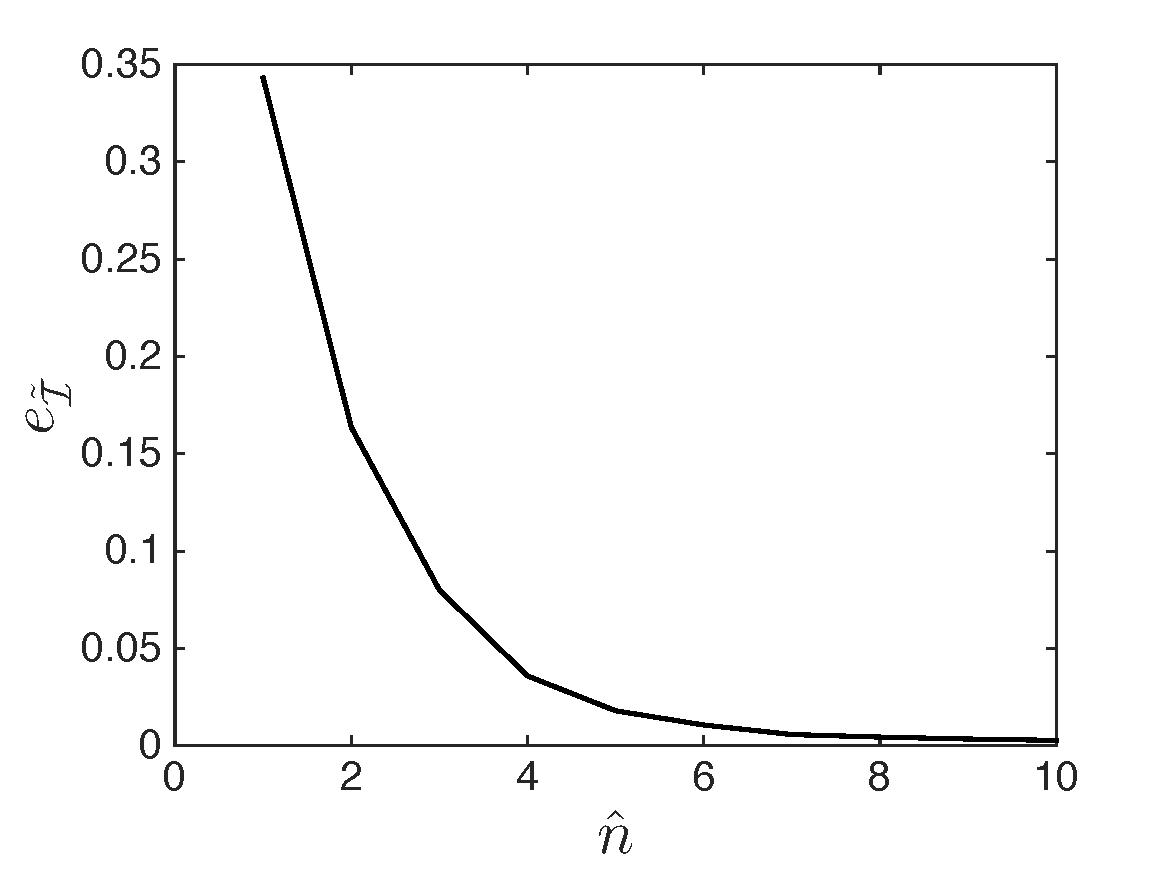
\includegraphics[height=0.35\columnwidth]{simpar_approx_err.pdf}
	}	
	\subfigure[Computation Ratio]
		{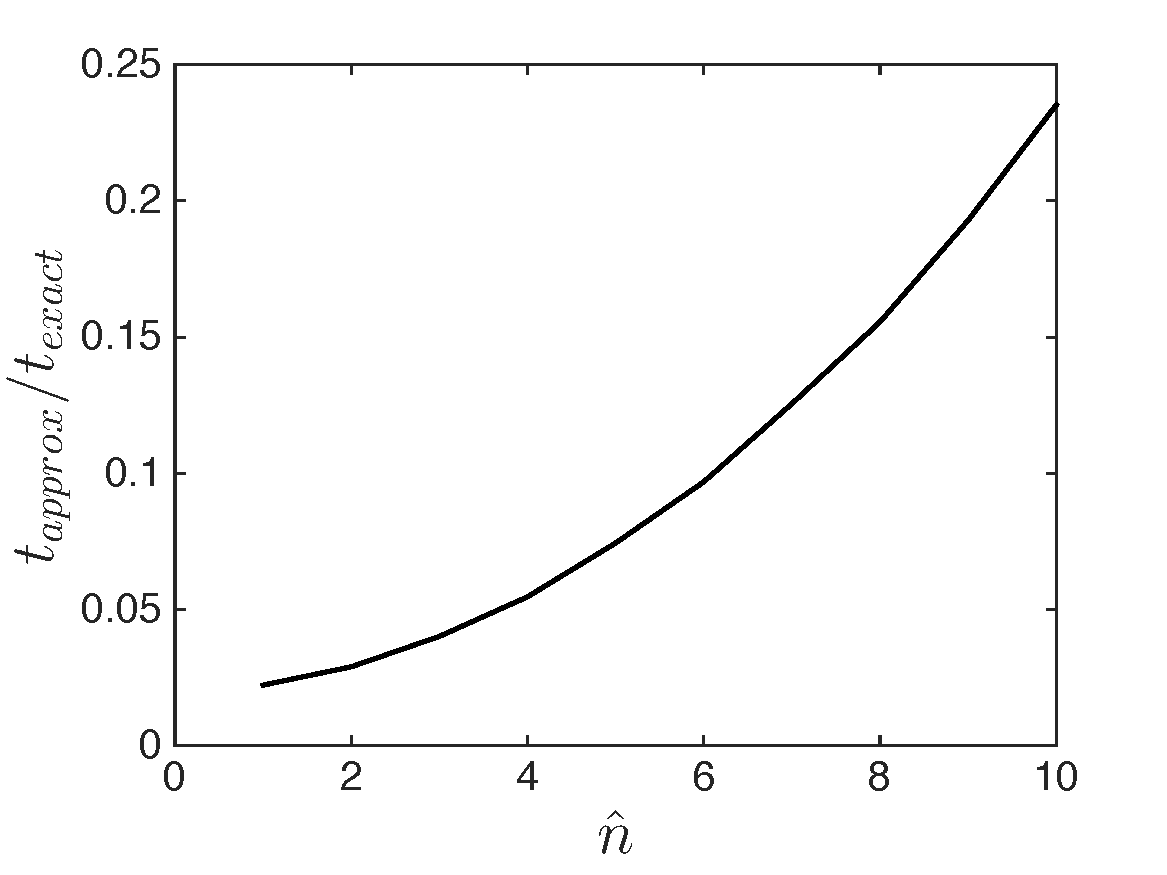
\includegraphics[height=0.35\columnwidth]{simpar_approx_t.pdf}
	}
}
\caption{The entropy error is decreased at the cost of increasing computation time in this Monte Carlo 1D measurement ray expected entropy case.}
\label{fig:ApproxJust}
\end{figure}



\section{Autonomous Exploration}

In this section, we develop an autonomous exploration scheme on a 2D map based on choosing movements that minimize entropy and avoid collisions.

\subsection{Pose Selection Optimization}

The robot pose at a future time step is selected to maximize \refeqn{ObjFun} over the search space $\Re^2\times\Sph^1$. We reduce the search by discretizing the search space in both position and attitude as follows. First, we choose $n_c$ candidate locations evenly-spaced along a circle of radius $\delta$, centered around the current location $x_t$, where the $c$-th candidate location is denoted $x_c\in\braces{x_1,x_2,\ldots,x_{n_c}}$, illustrated in Figure \ref{fig:OptProcess}. Any location that violates \refeqn{CollisionInequalityConstraint} is excluded to avoid collisions. For each candidate location, we consider $n_d$ evenly-spaced directions. The rays and attitudes at $x_c$ are denoted $\braces{z_{c,1},z_{c,2},\ldots,z_{c,n_d}}$ and $\braces{R_{c,1},R_{c,2},\ldots,R_{c,n_d}}$, respectively, where the scan with attitude $R_{c,d}$ might cover several ray directions depending on the sensor field of view (FOV). At $x_c$, we choose optimal attitude $R_c^*$ as the summation of the expected entropy changes covered by the scan,
\begin{align}
\label{eqn:FindRc}
&R_c^*=\argmax_{R_{c,d}}\sum_{z_{c,i}\in R_{c,d}\text{ FOV}}\bigg(H(P(m|X_{1:t},Z_{1:t}))\nonumber\\&\qquad\quad\quad\quad\quad-\text{E}[H(P(m|X_{1:t},Z_{1:t},x_c,z_{c,i}))]\bigg).
%\mathcal I_\text{ray}(x_c,z_{c,i})\right).
\end{align}


Therefore, the optimal attitude $R_c^*$ is given as a function of the location $x_c$. The objective function \refeqn{ObjFun} is computed by a summation about the $n_d$ rays as %\refeqn{Objective},
\begin{align}
\label{eqn:ObjFunApprox}
\mathcal I(x_c,R_c^*)&\approx \sum_{z_{c,i}\in R_{c}^*\text{ FOV}}\bigg(H(P(m|X_{1:t},Z_{1:t}))\nonumber\\&\ -\text{E}\left[H(P(m|X_{1:t},Z_{1:t},x_c,R_c^*,z_{c,i}))\right]\bigg),
\\
x_c^*&=\argmax_{x_c}\mathcal I(x_c,R_c^*).
\end{align}
%such that $X_c^*=\braces{x_c^*,R_c^*}$ is the optimal candidate over the discretized search space. Figure \ref{fig:OptProcess} illustrates this process.

\begin{figure}
\vspace*{0.08\columnwidth}
\centerline{
	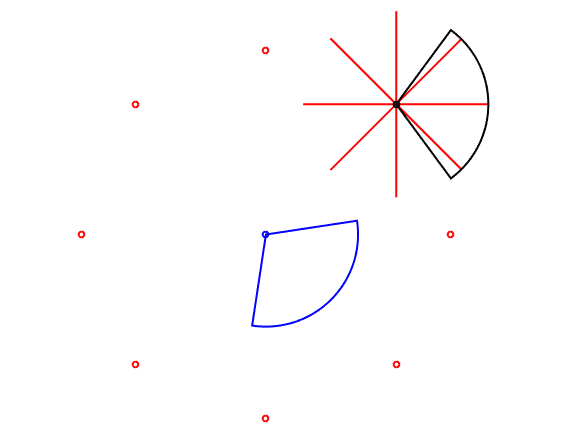
\includegraphics[height=0.35\columnwidth]{ExampleOptimalPose.png}
}
\begin{picture}(0,0)(0,0)
\setlength{\unitlength}{0.1\columnwidth}\scriptsize
\put(4.4,2.1){\color{blue}$X_t$}
\put(5.9,1.9){\color{red}$x_1$}
\put(2.9,2.0){\color{red}$x_5$}
\put(4.4,3.6){\color{red}$x_3$}
\put(4.4,0.6){\color{red}$x_7$}
\put(5.4,3.0){\color{red}$x_2$}
\put(3.3,3.1){\color{red}$x_4$}
\put(3.3,1.0){\color{red}$x_6$}
\put(5.4,1.0){\color{red}$x_8$}
\put(6.8,3.1){\color{red}$z_{2,1}$}
\put(4.5,3.1){\color{red}$z_{2,5}$}
\put(5.6,4.1){\color{red}$z_{2,3}$}
\put(5.6,2.2){\color{red}$z_{2,7}$}
\put(6.5,3.7){\color{red}$z_{2,2}$}
\put(4.9,3.8){\color{red}$z_{2,4}$}
\put(5.0,2.5){\color{red}$z_{2,6}$}
\put(6.5,2.5){\color{red}$z_{2,8}$}
\put(6.1,2.9){$X_c^*$}
\end{picture}
\caption{Initially, a robot (blue circle) views down and left (blue sector). Considering $n_c=8$ poses (red circles) as possible candidate locations to move next, $n_d=8$ sensor directions for each candidate are considered (red lines, only displayed on candidate location $c=2$). Then, the expected entropy of each ray is calculated. The scan (red sector) covering those rays with the largest expected entropy decreases is chosen for each candidate, and the best candidate $X_c^*$ (black circle: location, black sector: scan) is chosen to maximize information gain. Finally, Dijkstra's algorithm provides the collision-free motion between $X_t$ and $X_c^*$, and the process is repeated.
}
\label{fig:OptProcess}
\end{figure}


%In various modern sensors, such as the Kinect and LIDAR, several measurement rays are available simultaneously at any given scan. One may assume that each measurement ray provides independent information about the expected entropy change. Thus, one may add \refeqn{ObjFun} for each measurement ray. However, this assumption is often invalid in scenarios when a single grid cell is intersected by more than one measurement ray. For example, consider that the $i$-th cell is uncertain before considering $X_c$ as a future destination, i.e., $P(\mathbf{m}_i|X_{1:t},Z_{1:t})=0.5$ where H(0.5)=0.6931. Then, $\mathbf{m}_i$ is intersected by two candidate measurement rays $z_{c,1}$ and $z_{c,2}$, each with an expected entropy decrease of $0.4$. If summed, the total expected entropy value of this cell would be $-0.1069$, which is an impossible value because entropy is lower-bounded by $0$. The assumption is more flagrantly violated with increasing numbers of measurement rays passing through individual grid cells, motivating an alternative solution.
%
%Instead, when considering the $c$-th candidate, one may preselect a sample of evenly-spaced measurement rays, namely $\mathcal N=\braces{1,2,\ldots,n_d}$, deemed representative of the future scan. The spacing of these rays depends on the number of directions considered $n_d$, %which is chosen based on the desired predicted scan resolution and the spacing of the map grid cells, 
%where $n_d<n_z$ in general. Let these rays be denoted $\braces{z_{c,1},z_{c,2},\ldots,z_{c,n_d}}$, where the $d$-th direction satisfies $\braces{z_{c,d}\in\Re^2,\norm{z_{c,d}}=1}$. The goal is to consider enough rays that most grid cells covered by the scan are accounted by the rays of $\mathcal N$, while avoiding the case when multiple ray directions pass through any individual grid cell. In particular, one may choose a location for a pose, then find the expected entropy changes from various measurement rays. The $c$-th attitude $R_c^*$ is chosen such that the scan covers those measurement rays in the field of view (FOV) with the greatest sum of expected entropy decreases,
%\begin{align}
%\label{eqn:FindRc}
%R_c^*=\argmax_{R_c}\left(\sum_{z_{c,d}\in R_c \text{ FOV}}\mathcal I_\text{ray}(x_c,z_{c,l})\right).
%\end{align}
%In short, measurement rays in $n_d$ evenly-spaced directions around location $x_c$ are evaluated with \refeqn{DiscExpEntropyRay}. The attitude $R_c^*$ from \refeqn{FindRc} is determined from the maximum summation of ray expected information gains based off the $\mathcal N$ selected set, so $X_c=\braces{x_c,R_c^*}$ is selected as the candidate at $x_c$ to be compared with other candidates.


%\subsection{Motion Planning and Algorithm}
%
%The candidate pose locations may be determined several ways. For example in~\cite{CarDamKumCas15}, poses near frontiers as described in~\cite{Yam98} are selected as candidates. This choice is based on the intuition that poses near frontiers yield high expected entropy decreases, which is unproven. While frontier poses might produce effective candidates, they present a bias of candidates dependent on the geometry of the map according the robot knowledge. Thus, we choose pose candidates evenly-spaced in a circular pattern around the current location of the robot. Only should a candidate violate \refeqn{CollisionInequalityConstraint}, this candidate need not be considered.
%
%
%%Autonomous exploration is greedy, meaning that 
%We provide an algorithm pseudocode for autonomous exploration with occupancy grid applications. Consider $n_c$ candidate locations, namely $\braces{x_1,x_2,\ldots,x_{n_c}}$, evenly spaced around the current pose in a circular pattern of radius $\delta$, where the $c$-th candidate location is $x_{c}\in\Re^2$. %For each candidate location, consider $n_d$ evenly-spaced directions of the range sensor, namely $\braces{d_1,d_2,\ldots,d_{n_d}}$, where the $d$-th direction satisfies $\braces{d\in\Re^2,\norm{d}=1}$.

The objective function of the optimal pose $X_c^*=\braces{x_c^*,R_c^*}$ must satisfy $\mathcal I(X_c^*)\geq\mathcal I_\text{min}$ to avoid motions where little increased information is expected. 
If this condition is not satisfied, then $n_c$ and $\delta$ are multiplied by a scale function $\lambda>1$, candidates are chosen again, and $\mathcal I(X_c^*)$ is reevaluated.
Once the condition is satisfied, the robot must move to this pose while avoiding collisions subject to the inequality constraint \refeqn{CollisionInequalityConstraint}. In certain robotic applications, other cost parameters might be included in the optimization, e.g., driving time.

We choose Dijkstra's algorithm~\cite{Dij59} because it provides a relatively simple motion planning strategy from $x_t$ to $x_c^*$ that avoids local minima. Once the robot completes this motion, the entire process is repeated. This is summarized in the autonomous exploration pseudocode in Table \ref{tab:Alg_AutomousExploration}.


%The first pseudocode in table \ref{tab:Alg_AutomousExploration} outlines how a candidate pose is selected given an objective function. The second pseudocode in table \ref{tab:Alg_ObjFun}

\begin{table}
\vspace*{0.02\columnwidth}
\begin{tabular}{ l }
%  Define $n_c$: number of candidate locations\\
%  Define $n_d$: number of evenly-spaced measurement rays per candidate\\
  Given: $t=1$, $X_{1}$, $Z_{1}$, $P(m|X_{1},Z_{1})$ from the inverse sensor model\\
  TrajectoryComplete = false;\\
  while TrajectoryComplete = false\\
  \ \ if $X_{t+1}$ is unknown\\
  \ \ \ \ MotionPlanning = false;\\
  \ \ \ \ while MotionPlanning = false\\
  \ \ \ \ \ \ for $c = 1,2,\ldots,n_c$\\
  \ \ \ \ \ \ \ \ Candidate location: $x_{c}$ from evenly-spaced circle around\\
  \ \ \ \ \ \ \ \ $X_t$ with radius $\delta$;\\
  \ \ \ \ \ \ \ \ for $d=1,2,\ldots,n_d$\\
  \ \ \ \ \ \ \ \ \ \ Obtain reduced map $r_{c,d}$ with $n_{r_{c,d}}$ intersections\\
  \ \ \ \ \ \ \ \ \ \ through grid cells with depths $z_{c,d,1:n_{r,d}}$ from geometry;\\
  \ \ \ \ \ \ \ \ \ \ $\mathcal I_\text{ray}(x_c,z_{c,d})=\text{RayExpInfoGain}(x_c,P(r_{c,d}),z_{c,d,1:n_{r,d}})$;\\
  \ \ \ \ \ \ \ \ end for\\
  \ \ \ \ \ \ \ \ $R_{c}^*=\argmax_{R_c}\left(\sum_{z_{c,i}\in R_c \text{ FOV}}\mathcal I_\text{ray}(x_c,z_{c,i})\right)$;\\%\argmax_{R}{\sum_{d=1}^{n_d}\mathcal I_{\text{ray},c,d}|d\in\text{FOV}(R))}$;\\
  \ \ \ \ \ \ \ \ $\mathcal I(x_c,R_c^*)=\sum_{z_{c,i}\in R_c^* \text{ FOV}}\mathcal I_\text{ray}(x_c,z_{c,i})$;\\%\sum_{d\in \text{FOV}(R_c^*)}\mathcal I_{\text{ray}_{c,d}}$;\\
  \ \ \ \ \ \ end for\\
  \ \ \ \ \ \ $x_c^*=\argmax_{x_c}\mathcal I(x_c,R_c^*)$;\\
  \ \ \ \ \ \ $X_c^*=\braces{x_c^*,R_c^*}$;\\
  \ \ \ \ \ \ if $\mathcal I(X_c^*)<\mathcal I_\text{min}$\\
  \ \ \ \ \ \ \ \ $n_c=\text{round}(\lambda n_c)$;\\
  \ \ \ \ \ \ \ \ $\delta=\lambda \delta$;\\
  \ \ \ \ \ \ else\\
  \ \ \ \ \ \ \ \ Obtain $X_{t+1},X_{t+2},\ldots,X_{c}^*$ using Dijkstra's algorithm\\  \ \ \ \ \ \ \ \ planner and minimum rotation;\\
  \ \ \ \ \ \ \ \ Reset $n_c$ and $\delta$ to initial values;\\
  \ \ \ \ \ \ \ \ MotionPlanning = true;\\  
  \ \ \ \ \ \ end if\\
  \ \ \ \ end while\\
%  $X_c^*=\argmax_{X}$\mathcal I_{\text{ray},c
%  \ \ $\mathcal D\subset\braces{1,2,\ldots,n_d}$ represents scan coverage of candidate rays\\
%  \ \ The $c$-th pose candidate: $X_{c}=\braces{x_{c},R_{c}}$;\\
%   end for\\
%  $X_c^*=\argmin_{X_c}({\Delta H(X_c)}|X_c\in\braces{X_1,X_2,\ldots,X_{n_c}})$;\\
%  Motion planner generates a collision-free path between $X_t$ to $X_c^*$\\
%  Move to $X_{t+1}$, obtain $Z_{t+1}$, and find $P(m|X_{1:t+1},Z_{1:t+1})$;
  \ \ end if\\
  \ \ t = t+1;\\
  \ \ Obtain $P(m|X_{1:t},Z_{1:t})$ from the inverse sensor model;\\
  \ \ if map $m$ is completely explored\\
  \ \ \ \ TrajectoryComplete = true;\\
  \ \ end if\\
  end while


\end{tabular}
\caption{Autonomous Exploration via Expected Information Gain}
\label{tab:Alg_AutomousExploration}
\end{table}



\subsection{Numerical Example}

%Maximizing the proposed expected information gain serves as the objective for autonomous exploration. A robot begins in a completely uncertain environment, except for the grid cells inside the immediate vicinity the robot location. 
The robot models its surroundings with an occupancy grid with $15000$ cells where grid cell edges have length $\alpha=0.2$m, composing a map with dimensions $30\text{m}\times20\text{m}$. The initial probability $P(\mathbf{m}_i)=1\times10^{-10}\approx0$ (minimum value for free space) for grid cells covered by the circular robot of radius $0.1$m and $P(\mathbf{m}_i)=0.5$ for all other cells.
At each time step, the robot receives a measurement scan, where the probabilistic properties of the sensor are taken from~\cite{PirRutBisSch11,KhoElb12}. Then, the $n_c=8$ evenly-spaced candidate locations about a circle of radius $\delta=0.5$m around the current pose location are considered, where $n_d=32$ measurement rays are evenly-spaced about the candidate location.  When no current candidates yield expected information gains above $\mathcal I_\text{min}=2$, $\lambda=1.25$ is multiplied to $n_c$ and $\delta$. The motion of the robot is restricted to movement along cells satisfying \refeqn{CollisionInequalityConstraint} with $\beta=0.01$. Dijkstra's algorithm provides collision-free motion planning. %for robotic motion planning guides the robot through the environment without collision. 
The results are illustrated in Figure \ref{fig:AutonomousExploration}.


\begin{figure}
\centerline{
	\subfigure[Map at $t=50$sec]
		{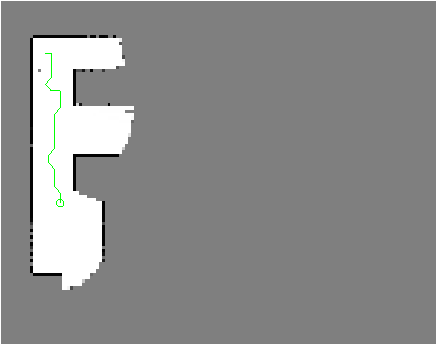
\includegraphics[height=0.3\columnwidth]{CDC16_t50.png}
	}	
	\hspace*{0.01\columnwidth}
	\subfigure[Map at $t=100$sec]
		{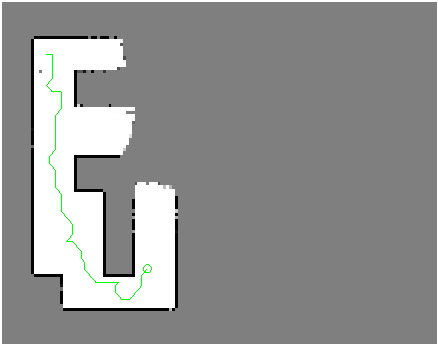
\includegraphics[height=0.3\columnwidth]{CDC16_t100.png}
	}
}
\centerline{
	\subfigure[Map at $t=150$sec]
		{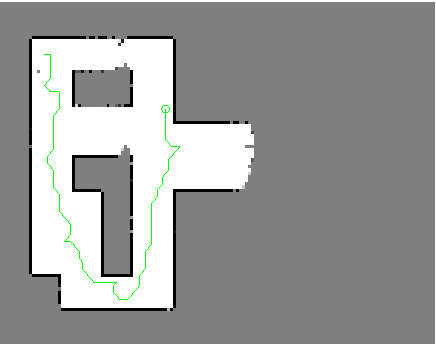
\includegraphics[height=0.3\columnwidth]{CDC16_t150.png}
	}	
	\hspace*{0.01\columnwidth}
	\subfigure[Map at $t=200$sec]
		{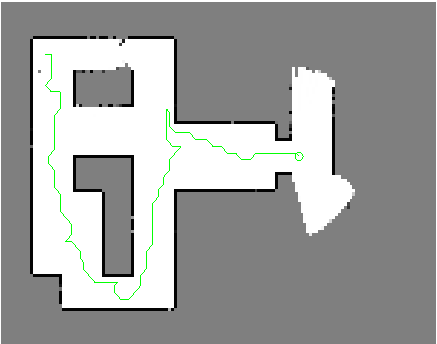
\includegraphics[height=0.3\columnwidth]{CDC16_t200.png}
	}
}
\centerline{
	\subfigure[Map at $t=250$sec]
		{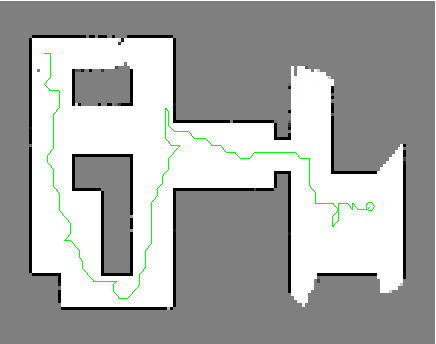
\includegraphics[height=0.3\columnwidth]{CDC16_t250.png}
	}	
	\hspace*{0.01\columnwidth}
	\subfigure[Map at $t=300$sec]
		{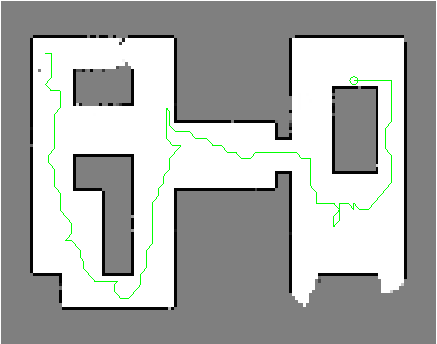
\includegraphics[height=0.3\columnwidth]{CDC16_t300.png}
	}
}
\centerline{
	\subfigure[Map at $t=350$sec]
		{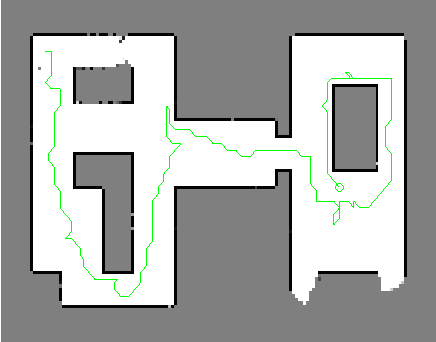
\includegraphics[height=0.3\columnwidth]{CDC16_t350.png}
	}	
	\hspace*{0.01\columnwidth}
	\subfigure[Map at $t=400$sec]
		{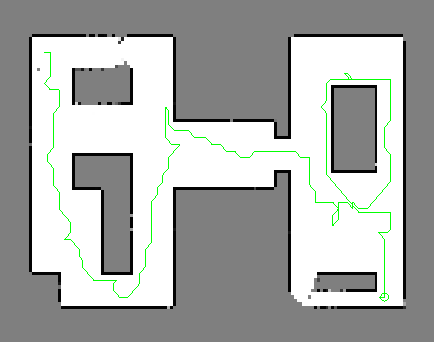
\includegraphics[height=0.3\columnwidth]{CDC16_t400.png}
	}
}\centerline{
	\subfigure[Map at $t=450$sec]
		{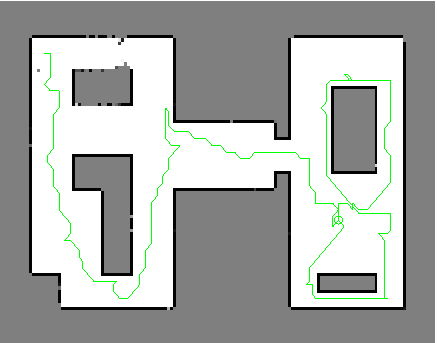
\includegraphics[height=0.3\columnwidth]{CDC16_t450.png}
	}	
	\hspace*{0.01\columnwidth}
	\subfigure[Map at $t=500$sec]
		{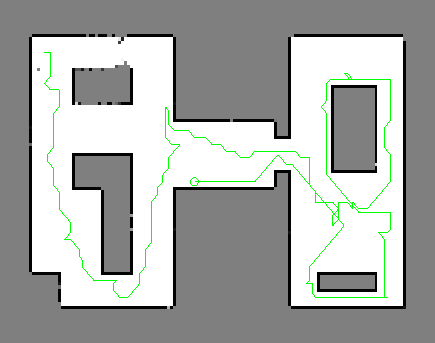
\includegraphics[height=0.3\columnwidth]{CDC16_t500.png}
	}
}
\caption{A robot (green circle, green marker of previous path) measures a room with a Kinect depth sensor to maximize map information gain. %The robot moves to maximize its information gain. %In the end, the robot is returning to the left room to gain more information about the uncertain regions it originally left behind.% The algorithms update the grid cells from uncertain (grey, $0.5$ occupancy probability) to either occupied (black, $1$ occupancy probability) or free (white, $0$ occupancy probability). Measured cells have occupancy probabilities closer to $0$ or $1$ as more information becomes available, and unmeasured cells remain near $0.5$, or uncertain.
%The exact inverse sensor model approach generates a more accurate result.
}
\label{fig:AutonomousExploration}
\end{figure}

Knowing only that the robot is inside free space at the beginning, the robot carefully navigates the environment while avoiding collisions. The robot motion is governed by a policy that maximizes the map information gain within its set of pose candidates, where the $\hat n=6$ is chosen to approximate the expected entropy of each ray. 
When running the exploration algorithm in Robot Operating System (ROS), the mean computation time is $0.0194$ seconds to determine the optimal future pose and complete Dijkstra's algorithm on the occupancy grid.
The computation times for this map reached roughly $1$ second at maximum, corresponding to rare cases when the robot is locally surrounded by a highly-certain environment; this task requires evaluating many more pose candidates and motion planning over a larger terrain. %Thus, the efficient computation makes the proposed autonomous exploration algorithm an effective strategy for real-time implementation.
%The median computation time for a single update is $0.7087$sec, though the mean is $1.3263$sec. 
%This discrepancy is due to high-computation outliers corresponding to cases when the robot is locally surrounded by a highly-certain environment; the robot must to traverse a large distance to learn information about another part of the map. Such a task requires evaluating many more pose candidates and motion planning over a larger terrain. 

Throughout the numerical example, the robot chooses numerous actions, based directly on their expected information gains, not frontiers or predicted measurement scans. If the obstacles were known a priori, the motion planning problem would yield a simpler path; however, the autonomous exploration is based on only the information of the map that the robot generates, so the motion planning must be reevaluated repeatedly. Even with these limitations, the robot explores the vast majority of reachable space in the $500$ second period. 


\section{Conclusions}

We developed a novel approach to autonomous exploration through an occupancy grid map based on a direct solution to expected entropy gain. Unlike common techniques based on frontiers or predicting measurement scans, the proposed approach is based on an expected value of the entropy directly. The approach is approximated with large improvements in computation and small losses in accuracy. A numerical example shows how a robot navigates an uncertain map governed by the proposed autonomous exploration algorithm.

%There are two important steps for future work. The first is to test the algorithm on a mobile robot navigating an uncertain environment while equipped with a Kinect depth sensor. The second is to extend the occupancy grid mapping and autonomous exploration to a multi-agent scenario.

\section*{Acknowledgment}
\addcontentsline{toc}{section}{Acknowledgment}
The authors would like to acknowledge Dr. Ira S. Moskowitz for helpful discussions on this topic.
%his helpful comments that served to improve the clarity of the theoretical contributions and writing of this paper. 



\bibliography{BibSources}
\bibliographystyle{IEEEtran}


%\begin{thebibliography}{99}
%
%\bibliography{BibSources}
%\bibliographystyle{IEEEtran}
%
%\end{thebibliography}

% Henry Carrillo

%\begin{thebibliography}{99}
%
%\bibitem{c1}
%J.G.F. Francis, The QR Transformation I, {\it Comput. J.}, vol. 4, 1961, pp 265-271.
%
%\bibitem{c2}
%H. Kwakernaak and R. Sivan, {\it Modern Signals and Systems}, Prentice Hall, Englewood Cliffs, NJ; 1991.
%
%\bibitem{c3}
%D. Boley and R. Maier, "A Parallel QR Algorithm for the Non-Symmetric Eigenvalue Algorithm", {\it in Third SIAM Conference on Applied Linear Algebra}, Madison, WI, 1988, pp. A20.
%
%\end{thebibliography}

\end{document}
